\subsection{Erfüllung der funktionalen Anforderungen}

Wie zu erkennen ist, ließen sich die nicht funktionalen Anforderungen ausreichend erfüllen.
Im Folgenden soll nun überprüft werden, ob dies auch auf die funktionalen Anforderungen zutrifft.

Dafür sollen diese hier aufgelistet und dann einzeln auf diese eingegangen werden.
Dabei soll durch Screenshots die tatsächliche Realisierung angedeutet werden.

\subsubsection{FNC\#01 – Definition eines Straßenlayouts}

Die Implementation der Anforderung \refgoal{fnc:define_layout} ist vor allem im Datenmodell zu erkennen, insofern durch dieses das eigentliche Raster repräsentiert worden ist.
Um diese Anforderung zu erfüllen, wurden verschiedenste Kachel-Modelle erworben und mit den jeweiligen Spur Informationen versehen.

Durch das gleichmäßige Raster können, wie vorgesehen, sowohl Agenten als auch Nutzer mit ihm leicht umgehen.
Ein Beispiel dafür, wie ein Agent dieses Raster nutzen kann, ist im vorgefertigten Random Exit Driver beigelegt.
Dieser nutzt das Kachelmodell, um dadurch effiziente Caches für die Wegfindung aufzubauen.
Die zeitlich praktikable Implementation dieses Caches funktionierte hier primär durch diese Limitierung.

Für den Nutzer ist diese Art des Modells ebenfalls einfacher, da das Raster leichter nachzuvollziehen und zugänglicher ist als eine Freiform-Positionierung.
Zusätzlich muss hierfür der Nutzer nicht so geschickt sein und macht dadurch weniger Fehler bei der Definition.
Dies ist auch in der Ausführung für die Anforderung \refsec{sec:check-fnc-3} zu erkennen.

Für die Erstellung eines solchen Layouts wird der Nutzer anfangs vor die Wahl gestellt, ob er ein anderes Layout als Grundlage verwenden möchte.
Er kann dabei aus bereits existierenden Layouts wählen und diese dadurch erweitern bzw. nach Belieben anpassen.
Sollte er das nicht wollen, kann er, wie in Abbildung \refimg{fig:layout-base} zu erkennen, auch mit einem leeren Layout fortfahren.

\begin{figure}[htb]
    \centering
    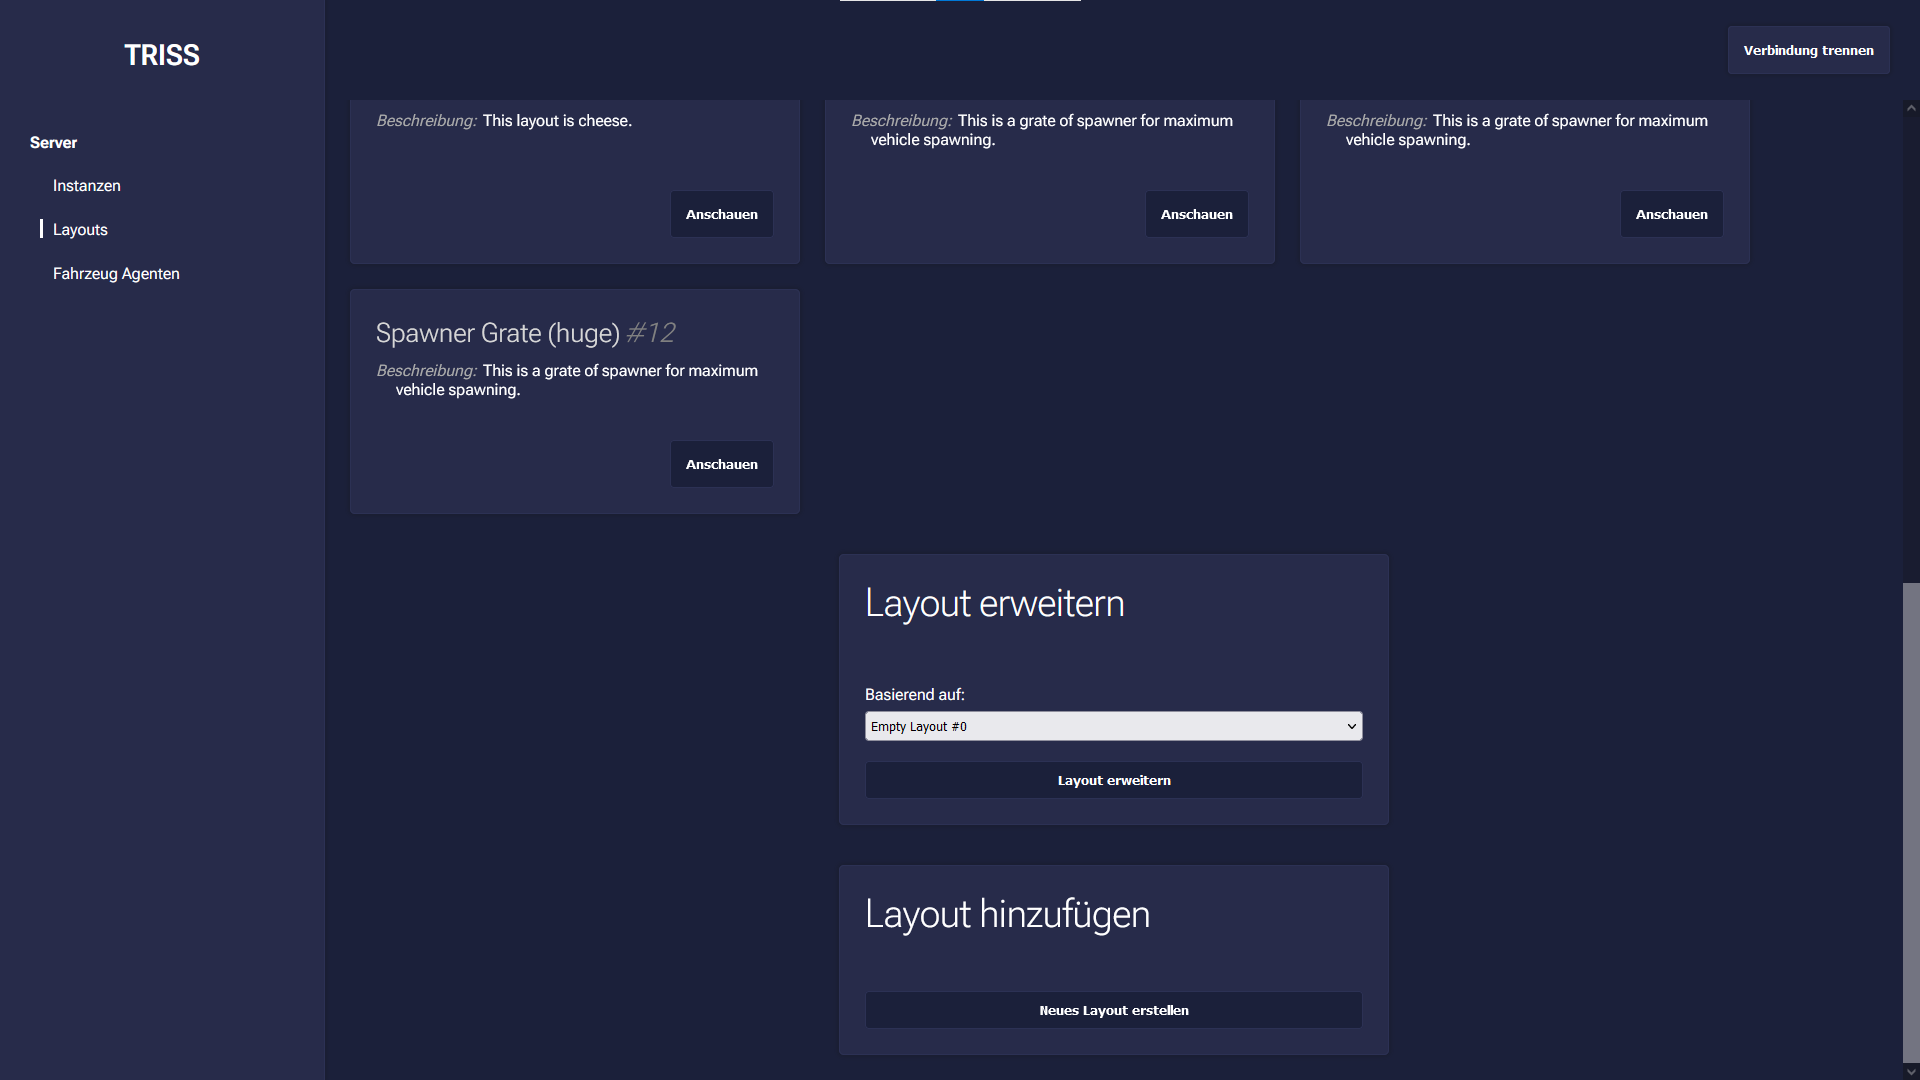
\includegraphics[scale=.25,center]{medien/screenshots/layout-base.png}
    \caption{Layout Grundlage auswählen}
    \ownsource
    \label{fig:layout-base}
\end{figure}

Nach dem Auswählen ist er in der Lage, die Metainformationen zu hinterlegen und, wie in \refgoal{fnc:configure_layout} beschrieben, Kacheln zu platzieren.

\FloatBarrier

\subsubsection{FNC\#02 – Inspektion eines Straßenlayouts}

Diese Anforderung ließ sich mithilfe der bereits genannten Modelle sowie mit der three.js Bibliothek voll umsetzen.
Alle auf dem Server gespeicherten Layouts werden für den Nutzer in einer Liste, wie in \refimg{fig:choose-layout} abgebildet, dargestellt.
In dieser Liste wird für jede Entität der Name, die Identifikationsnummer sowie die Beschreibung angezeigt.

\begin{figure}[htb]
    \centering
    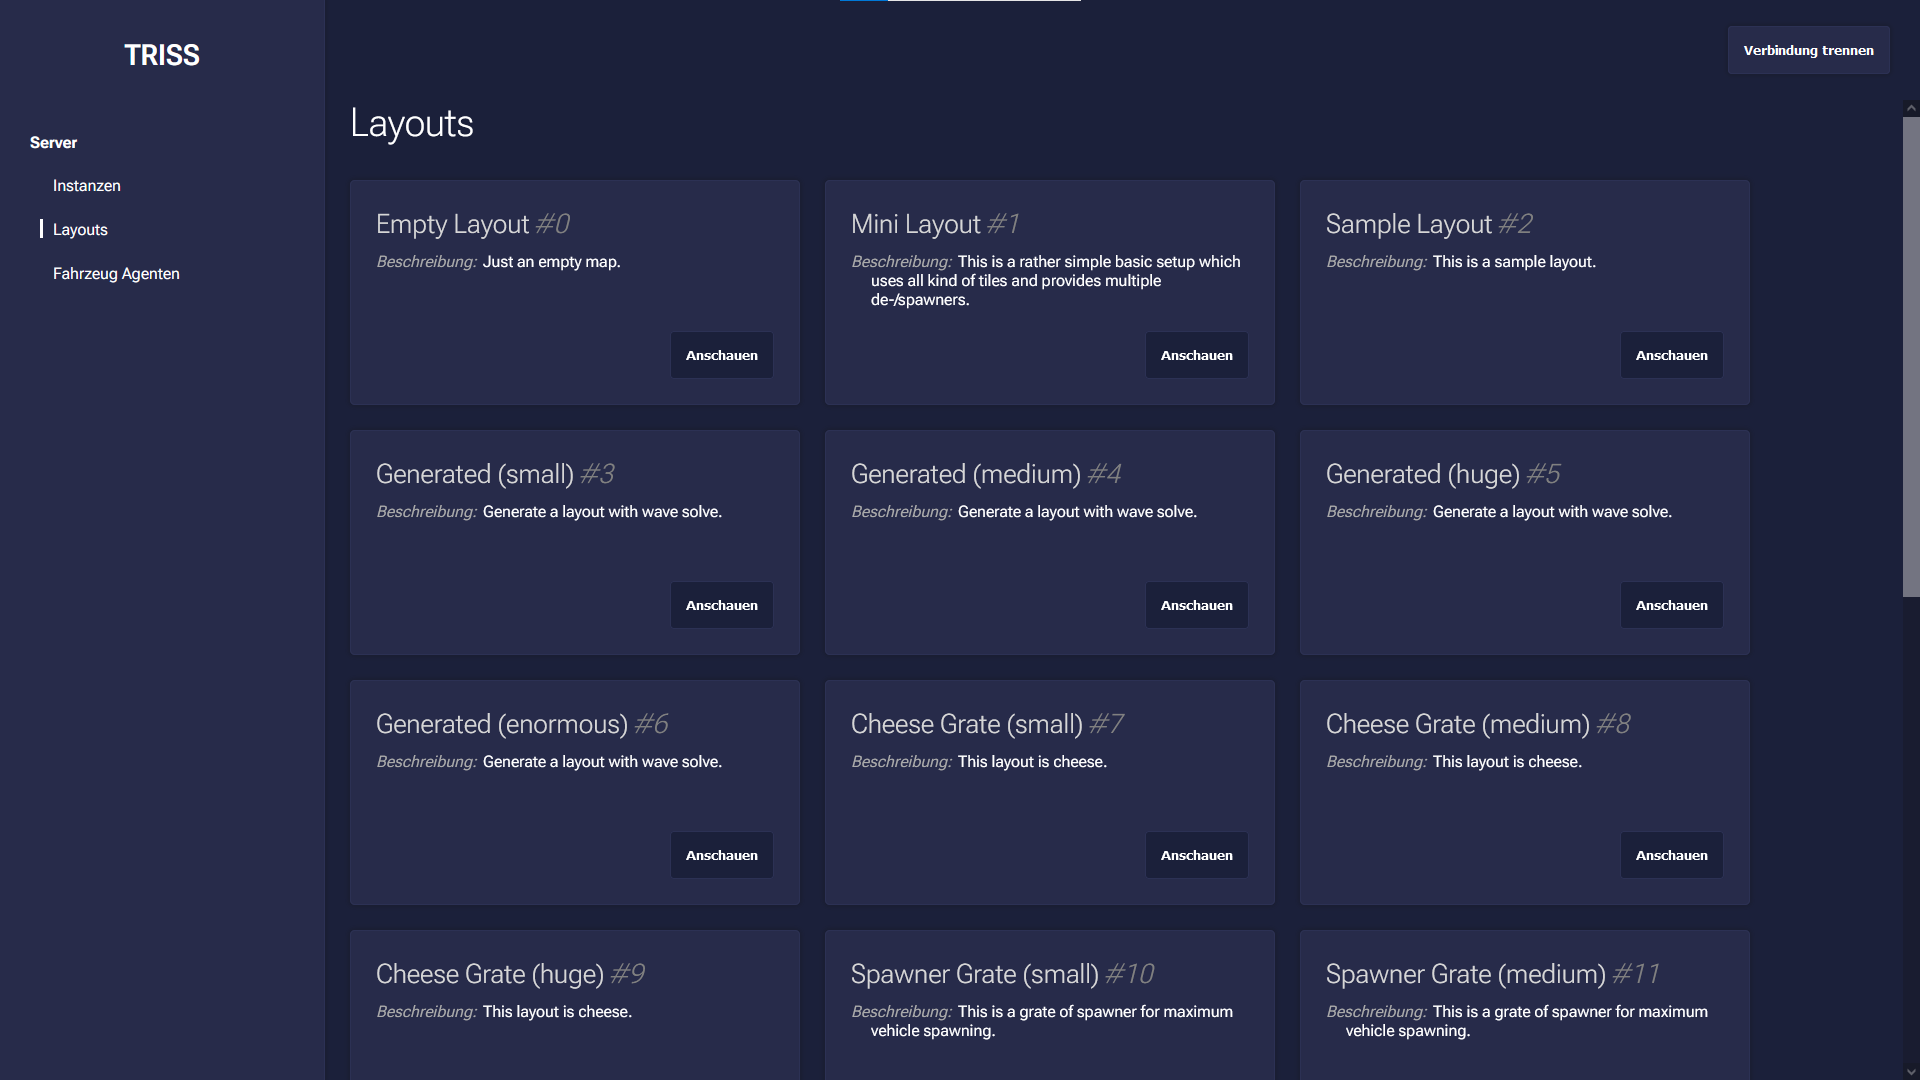
\includegraphics[scale=.25,center]{medien/screenshots/choose-layout.png}
    \caption{Layout auswählen}
    \ownsource
    \label{fig:choose-layout}
\end{figure}

Durch das Drücken auf \textit{Anschauen} wird das Layout für das Betrachten ausgewählt.
Damit dieses dargestellt werden kann, wird dieses zuerst vom Server bezogen und im Anschluss an die Komponente für die Darstellung weitergereicht um dann die Darstellung, wie in \refimg{fig:layout-view} zu sehen, zu erzeugen.

\begin{figure}[htb]
    \centering
    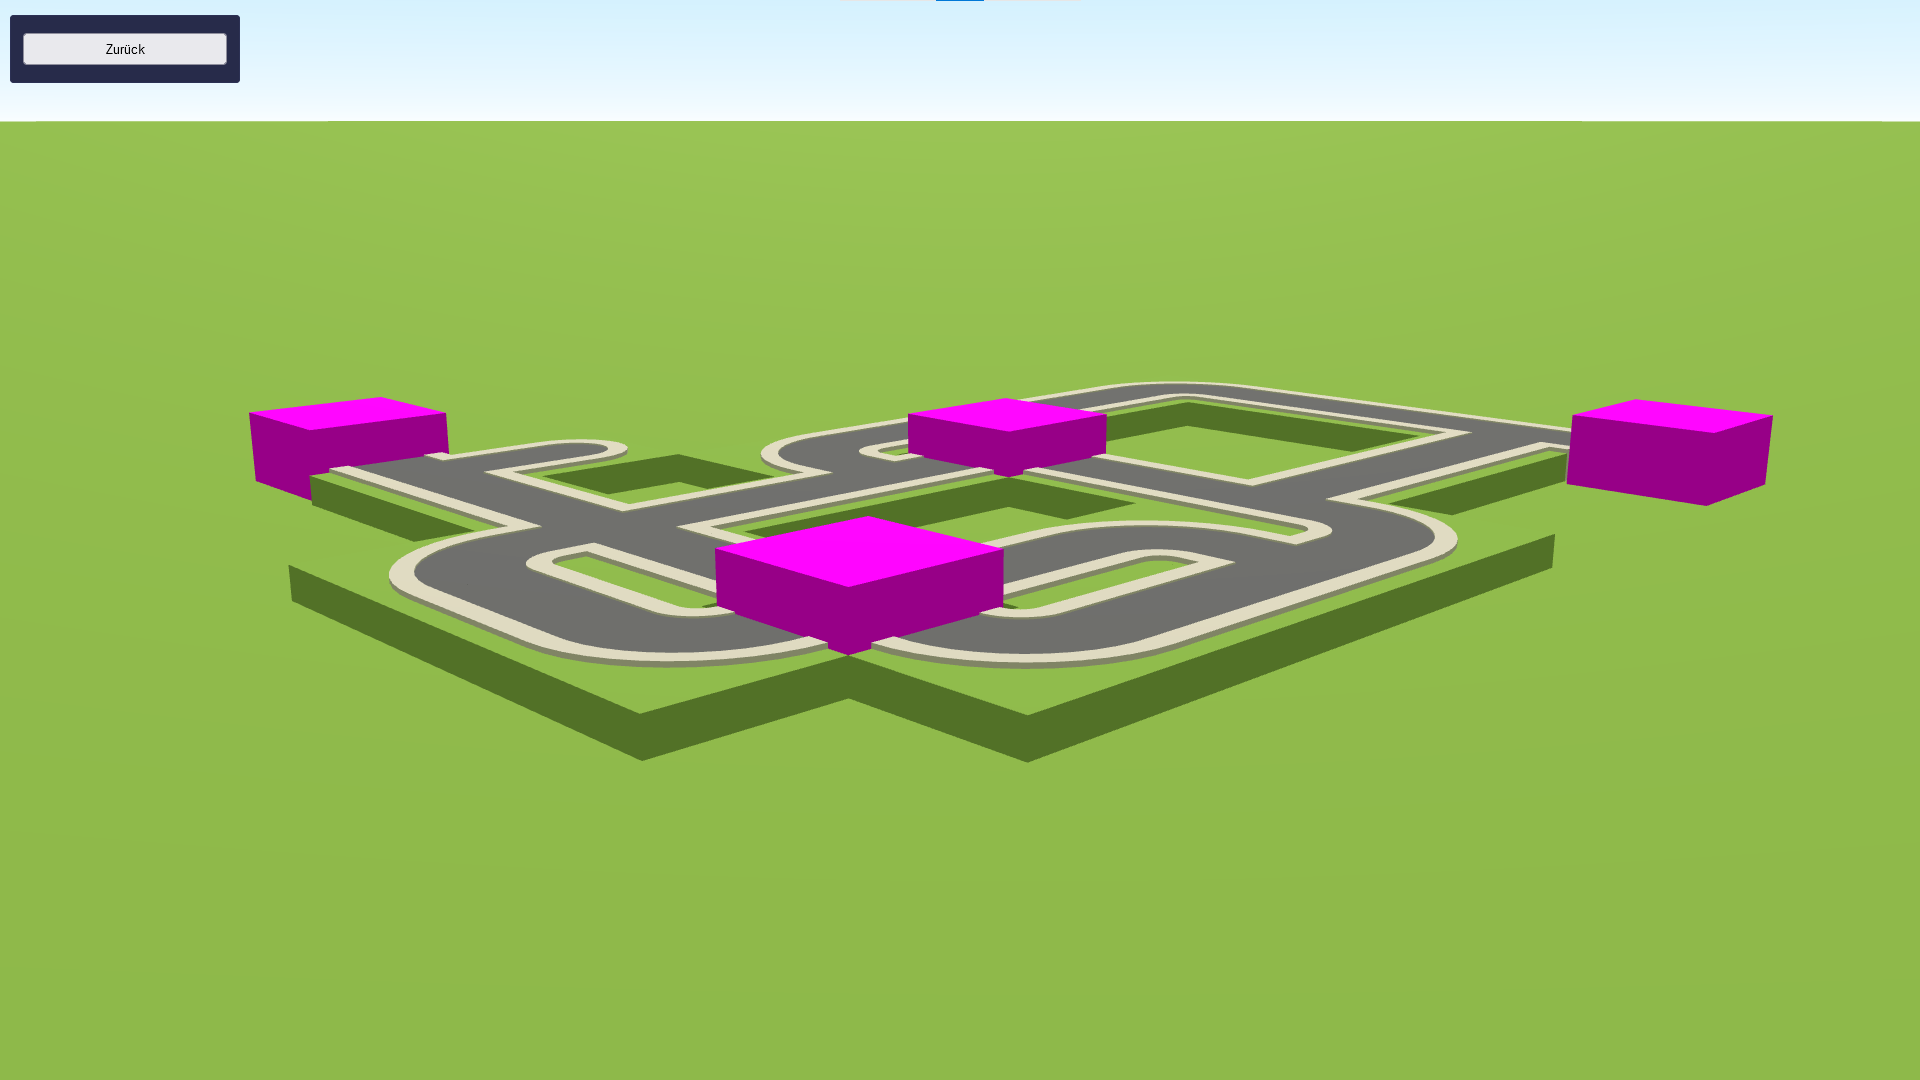
\includegraphics[scale=.25,center]{medien/screenshots/layout-view.png}
    \caption{Layout inspizieren}
    \ownsource
    \label{fig:layout-view}
\end{figure}

In dieser kann man dann via der Maus die Ansicht rotieren und mit dem Mausrad die Kamera herein- und herausbewegen.
Somit lässt sich das Layout frei inspizieren und nachvollziehen.

%\FloatBarrier

\subsubsection{FNC\#03 – Platzierung einer Kachel} \label{sec:check-fnc-3}

Für das Platzieren der Kachel wurde eine ähnliche Ansicht erstellt wie die, die für die Anforderung \refgoal{fnc:inspect_layout} verwendet worden ist.

So kann der Nutzer auch hier mit der Maus die Kamera frei bewegen.
Zusätzlich erhält er weitere UI-Elemente, wie in \refimg{fig:place-ui} abgebildet, durch die er in der Lage ist, Kacheln zu platzieren.

\begin{figure}[htb]
    \centering
    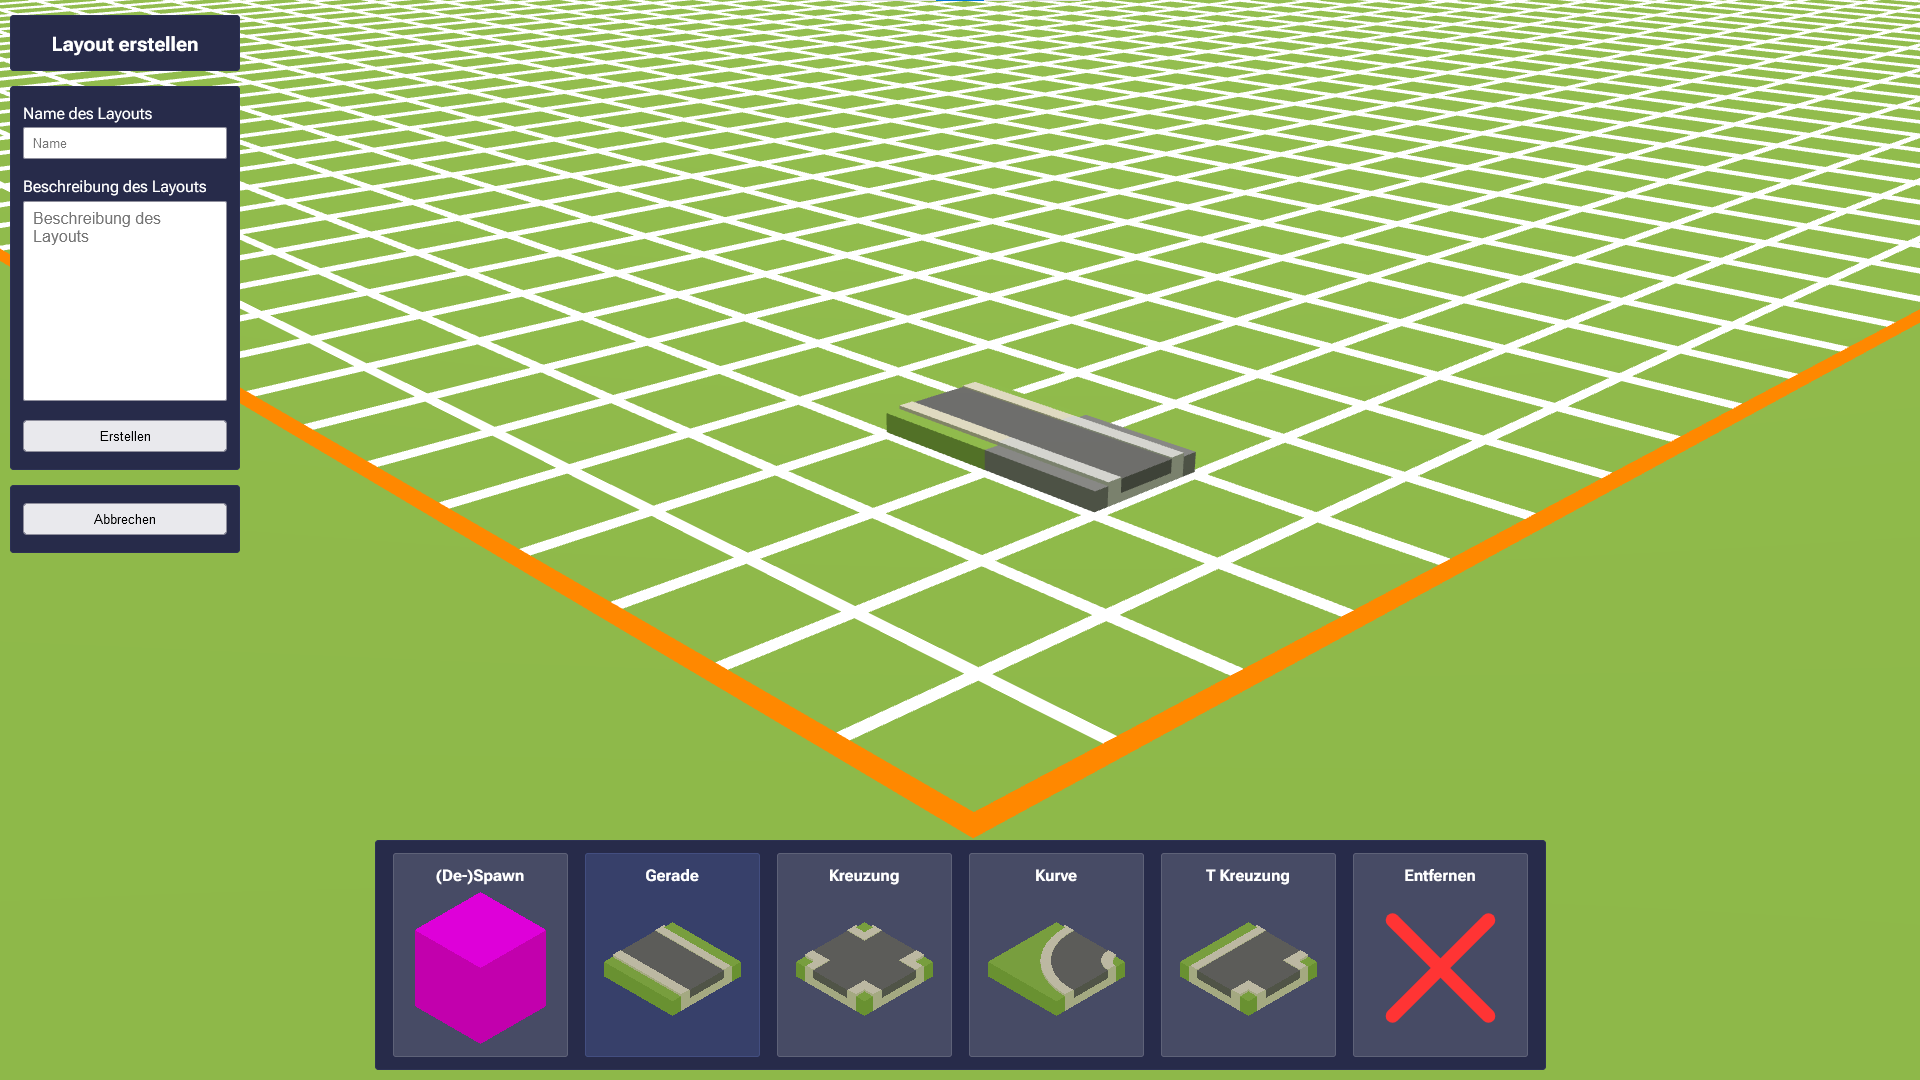
\includegraphics[scale=.25,center]{medien/screenshots/place-ui.png}
    \caption{UI für die Erstellung eines Layouts}
    \ownsource
    \label{fig:place-ui}
\end{figure}

Dabei kann der Nutzer über die Elemente auf der linken Seite die Metadaten für das Layout spezifizieren und mit der Auswahlliste in der unteren Hälfte festlegen, welche Wirkung der Linksklick aktuell hat.

Bei allen Optionen, bis auf die \textit{Entfernen} Funktion, hat der Nutzer beim Bewegen der Maus über das Raster eine schattierte Version der ausgewählten Kachel, die dem Cursor folgt.
Wenn man dann via Linksklick die Kachel platziert, nimmt diese ihre korrekte Farbe/Textur an und verbleibt an dem Ort, an dem sie vorher dargestellt worden ist.

So lassen sich Kacheln auch überschreiben und via den Tasten \enquote{,} und \enquote{.} rotieren.
Durch die letzte Option kann der entfernen Modus aktiviert werden, wodurch bei einem Linksklick die Kachel wieder entfernt wird.

Diese Implementation sollte die komplette Anforderung erfüllen, auch wenn hier nicht alle Kacheln für das Platzieren zur Verfügung gestellt werden.

%\FloatBarrier

\subsubsection{FNC\#04 – Spezifikation eines Agenten}

Die Spezifikation ist aufwendiger zu implementieren gewesen und hat sich im Verlauf der Entwicklung auch zwei Mal grundsätzlich verändert.

Bei der finalen Implementation ist statt den Metafeldern nur noch der Upload vorhanden.
Dieser erwartet nun im Wurzelverzeichnis eine \textit{package.json}, die den Namen und die Beschreibung beinhaltet und dann aus dieser heraus gelesen wird.
Dies soll eine Dopplung von Informationen verhindern und damit Änderungsanomalien vorbeugen.

Die Dateien werden dann in den Workspace geschrieben und via Yarn installiert, das heißt, dass diese nun korrekt externe Abhängigkeiten haben können und damit dem Agenten noch mehr Freiheiten geben, wie dieser intern funktioniert.

Die restliche Spezifikation ist, wie in dem vorangegangenem Evaluationskapitel zu erkennen, so wenig einschränkend wie möglich.

\subsubsection{FNC\#05 – Betrieb einer Simulation}

Diese Anforderung konnte ziemlich genau so implementiert werden, wie es vorgesehen war.
Vor allem auf den Aspekt der Isolation konnte hier eingegangen werden, indem mit Workern ein eigener Kontext geschaffen worden ist und dadurch, selbst wenn dieser viele externe Bibliotheken benötigt, diese nicht direkt für alle geladen werden.

\subsubsection{FNC\#06 – Inspektion einer Simulation}

Die Umsetzung dieser Anforderung war die aufwendigste und vielseitigste.
Das lag vor allem daran, dass sie zusammen mit der nicht funktionalen Anforderung \refgoal{qlt:rendering_efficiency} mehrere Gesichtspunkte hatte, die im Zusammenspiel eine sehr solide Implementation erforderten, um sie zu erfüllen.
Dies ist allerdings, wie auch bereits in dem Abschnitt \refsec{sec:application_efficiency} beschrieben, sowohl im Hinblick auf die Leistungs- als auch auf die Funktionalen-Merkmalen gelungen.

\begin{figure}[htb]
    \centering
    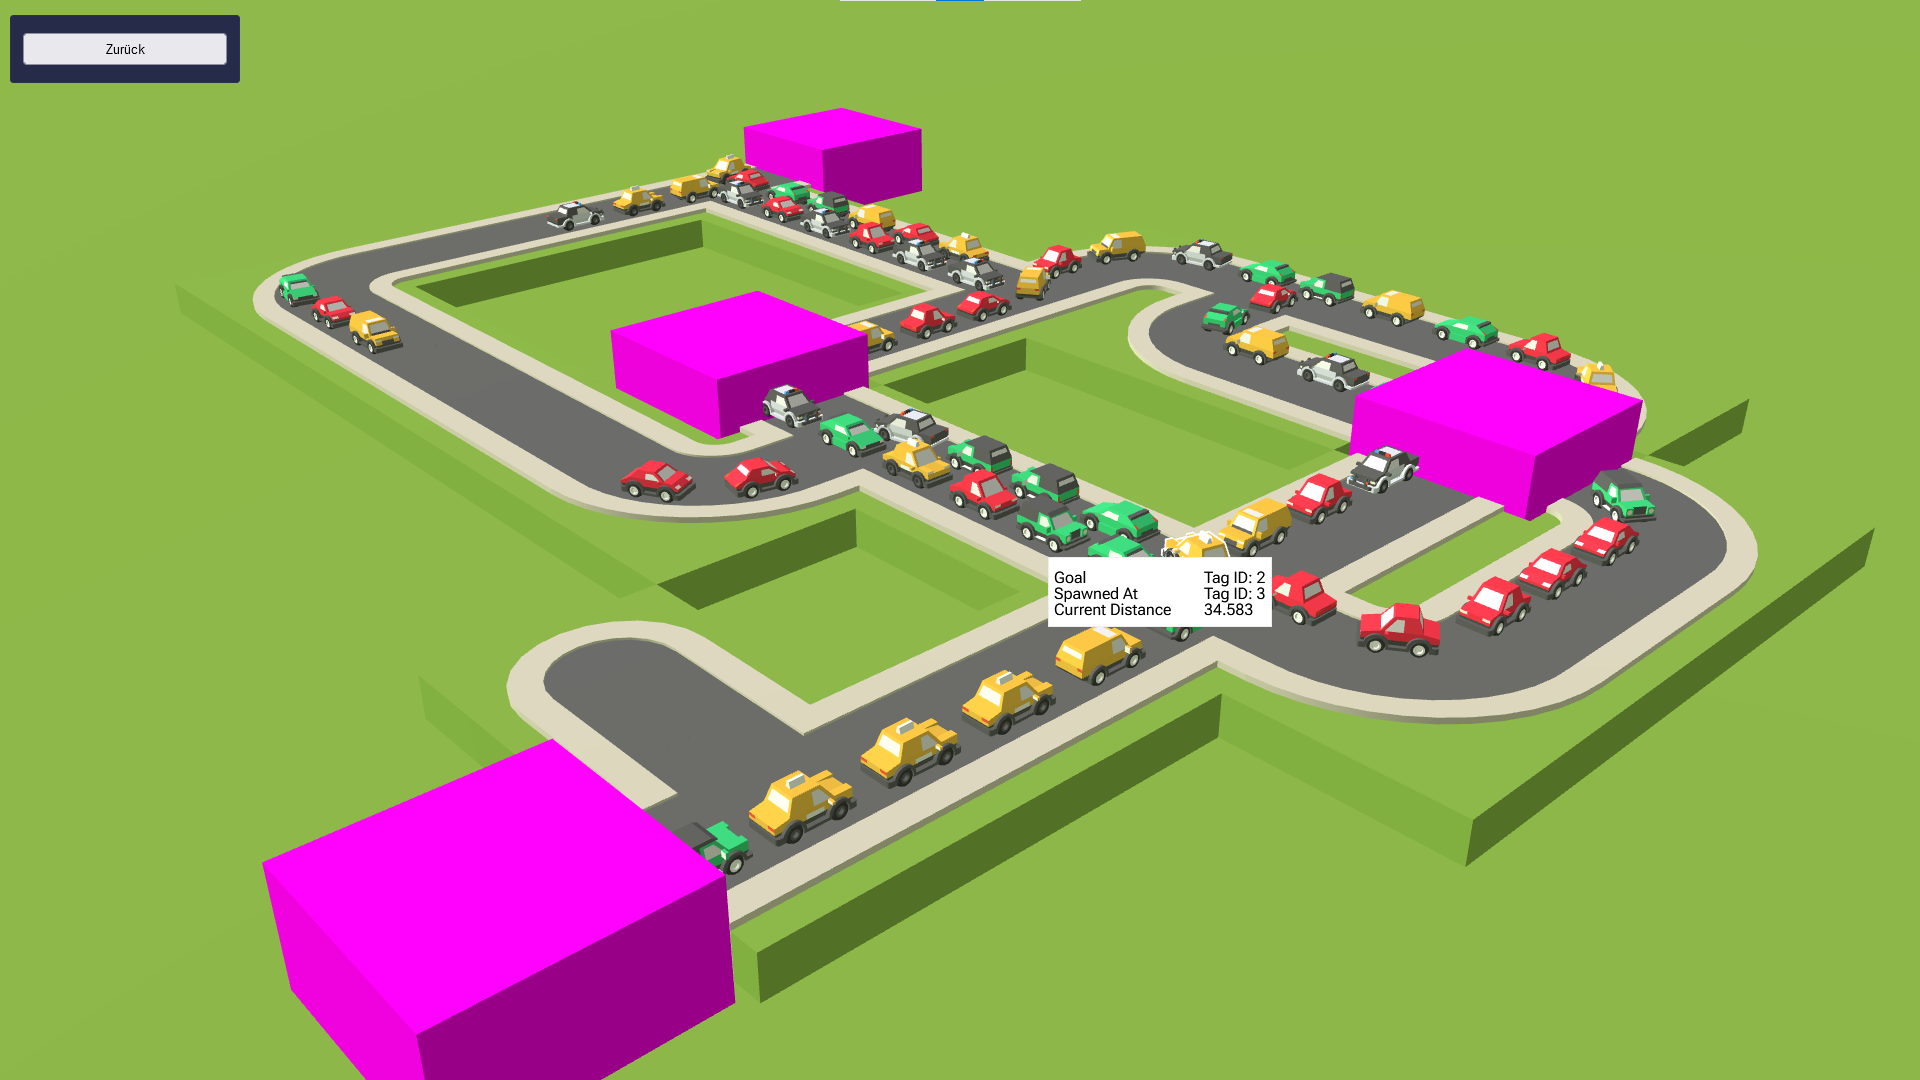
\includegraphics[scale=.25,center]{medien/screenshots/instance-view.png}
    \caption{Darstellung einer Instanz}
    \ownsource
    \label{fig:instance-view}
\end{figure}

Dies gelang vor allem deshalb, weil sich bei der Implementation von dem Node System\footnote{\url{https://docs.blender.org/manual/en/3.2/compositing/introduction.html}} \footnote{\url{
https://docs.blender.org/manual/en/3.2/render/shader_nodes/index.html}} der Blender Suite inspiriert worden lassen ist und dadurch die Implementation so abstrahiert werden konnte, dass sich die einzelnen Komponenten zielführend verbessern ließen.

Zusätzlich lassen sich durch die Export-Schnittstelle des Agenten auch Daten in Echtzeit an dem Fahrzeug anbringen und darstellen (siehe \refimg{fig:instance-view}), wodurch das Nachvollziehen des Verhaltens dieser Instanz noch einfacher wird.

Die gesamte Darstellung ist, wie gewünscht, in Echtzeit mit einer kontinuierlich guten Performance und einer hohen Bildwiederholrate möglich.

Insgesamt war die Implementation dieses Abschnitts die aufwendigste, insofern sie viele Komponenten umfasste und eine sehr solide Implementation voraussetzte.
Jedoch ist es gelungen, auch diese Anforderung wie gewünscht umzusetzen.
